\documentclass{article}

\usepackage[margin=0.95in]{geometry}
\usepackage{graphicx}
\graphicspath{ {images/} }


\title{Godel's Incompleteness Theorem}
\author{Krishna Agrawal, 19111031}
\date{\today}

\begin{document}
\maketitle

\subsection*{Introduction}
Gödel's incompleteness theorems are two theorems of mathematical logic that are concerned with the limits of provability in formal axiomatic theories. The first incompleteness theorem states that no consistent system of axioms whose theorems can be listed by an effective procedure is capable of proving all truths about the arithmetic of natural numbers. For any such consistent formal system, there will always be statements about natural numbers that are true, but that are unprovable within the system. The second incompleteness theorem, an extension of the first, shows that the system cannot demonstrate its own consistency.  


\subsection*{Systems: completeness, consistency, and effective axiomatization:}

The incompleteness theorems apply to formal systems that are of sufficient complexity to express the basic arithmetic of the natural numbers and which are consistent, and effectively axiomatized.

In general, a \textbf{\emph{formal system}} is a deductive apparatus that consists of a particular set of axioms along with rules of symbolic manipulation that allow for the derivation of new theorems from the axioms.
A formal system is said to be effectively \textbf{\emph{axiomatized}} if its set of theorems is a recursively enumerable set.
A set of axioms is \textbf{\emph{complete}} if, for any statement in the axioms' language, that statement or its negation is provable from the axioms.
A set of axioms is \textbf{\emph{consistent}} if there is no statement such that both the statement and its negation are provable from the axioms, and inconsistent otherwise.

\subsubsection*{First Incompleteness Theorem:} "Any consistent formal system \emph{F} within which a certain amount of elementary arithmetic can be carried out is incomplete; i.e., there are statements of the language of \emph{F} which can neither be proved nor disproved in \emph{F}." \\

The unprovable statement $G_{F}$ referred to by the theorem is often referred to as "the Gödel sentence" for the system \emph{F}. 

\subsubsection*{Second Incompleteness Theorem:} 
For each formal system \emph{F} containing basic arithmetic, it is possible to canonically define a formula Cons(\emph{F}) expressing the consistency of \emph{F}. This formula expresses\\

 "Assume \emph{F} is a consistent formalized system which contains elementary arithmetic. Then 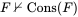
\includegraphics[scale=.6]{image} " \\\\
 The standard proof of the second incompleteness theorem assumes that the provability predicate $Prov_{A}$(\emph{P}) satisfies the Hilbert–Bernays provability conditions. 

\subsubsection*{Summary}
Gödel's incompleteness theorems were the first of several closely related theorems on the limitations of formal systems. Gödel's second incompleteness theorem is stronger than the first incompleteness theorem because the statement constructed in the first incompleteness theorem does not directly express the consistency of the system. Also, the proof of the second incompleteness theorem is obtained by formalizing the proof of the first incompleteness theorem within the system \emph{F} itself. These results, are important both in mathematical logic and in the philosophy of mathematics. 

\end{document}